\documentclass[11pt]{article}
\usepackage[utf8]{inputenc}
\usepackage{amsmath}
\usepackage{titlesec}
\usepackage{titling}
\usepackage{geometry}
\usepackage{graphicx}
\usepackage{hyperref}
\usepackage{fancyhdr}
\usepackage{wallpaper}
\usepackage{afterpage} 
\usepackage{pagecolor} 
\usepackage{multirow}
\usepackage{wrapfig}
\usepackage{lipsum} % for dummy text
\usepackage{url}
\usepackage[toc,page]{appendix}
\usepackage{mdframed}
\usepackage{pgfgantt}
\usepackage{tabularx}


% Define colors
\usepackage{xcolor}
\definecolor{myblue}{RGB}{33, 66, 99}
\definecolor{mygray}{RGB}{169, 169, 169}
\definecolor{darkbluegrey}{RGB}{44, 62, 80} 

% Page styling
\pagestyle{fancy}
\fancyhf{}
\renewcommand{\headrulewidth}{0pt}
\renewcommand{\footrulewidth}{0pt}
\fancyfoot[C]{\thepage}
\renewcommand{\familydefault}{\sfdefault}

% Define a command for section headers
\titleformat{\section}
  {\color{myblue}\normalfont\Large\bfseries}
  {\color{myblue}\thesection}{1em}{}

% Define a command for subsection headers
\titleformat{\subsection}
  {\color{myblue}\normalfont\large\bfseries}
  {\color{myblue}\thesubsection}{1em}{}

% Adjust page margins
\geometry{a4paper, margin=1in}

% make references clickable
\hypersetup{
    colorlinks=true,
    linkcolor=blue,
    filecolor=magenta,      
    urlcolor=cyan,
}

\begin{document}

% Change the background color of the first page
\pagecolor{darkbluegrey}
\afterpage{\nopagecolor}

% Add a background image
\ThisCenterWallPaper{0.75}{./image/spike_brain.png}

\begin{titlepage}
  \vspace*{\stretch{1}}
  \begin{center}
    \textcolor{white}{\textbf{\Huge Description of Work}}\\ % changed text color to white
    \vspace{1cm}
    \textcolor{white}{\Large Sound Detection and Classification\\using Spiking Neural Networks} % changed text color to white
    \vspace{3cm}
  \end{center}
  \vspace*{\stretch{2}}
  \begin{center}
    \textcolor{white}{ % changed text color to white
      \textbf{COURREGE Téo}\\
      \textbf{GANDEEL Lo'aï}\\
      \vspace{1cm}
      \Large Date: \today}
  \end{center}
  \vspace*{\stretch{1}}
\end{titlepage}

\newpage

\tableofcontents

\pagebreak

\section{Introduction}

Our project addresses the challenge of applying spiking neural networks (SNNs) to audio classification in the field of spiking neural network (SNN) research. This report provides an overview of our initial progress in this area. Our project specifically addresses the problem of audio classification within the broader context of SNNs.

Before delving into the details, we outline key aspects including preprocessing, data manipulation/augmentation, initial model implementations, and a look at preliminary results.

Using audio data primarily from the \href{https://research.google.com/audioset/}{Google AudioSet} database, our work involves preprocessing, which includes conversion of signals to image representations, feature extraction, and consideration of encoding schemes suitable for SNNs. Challenges related to data quality, context, and labeling complexity prompted the exploration of data augmentation strategies to improve model robustness.

In the following sections, we will elaborate on the organizational structure of our project, the technical environment utilized, a detailed account of the work accomplished, challenges faced and solutions implemented, concluding with a reflection on our achievements and future perspectives.

Chat:

In the following sections, this report will delve into the organization that underpin our project. A detailed examination of the technical environment, including the computational tools, software frameworks, programming languages, and relevant documentation, will shed light on the methodological underpinnings of our research.

This is followed by an account of the work performed. The technical and theoretical advances made during the project are highlighted. The challenges faced, ranging from technical hurdles to conceptual complexities, will be discussed in detail, along with the strategic solutions developed to overcome these obstacles. The section will also reflect on the usefulness of the feedback received during the initial stages of the project presentation.

Finally, the report will conclude with a discussion of our achievements, highlighting the areas where significant progress has been made. We will outline our future perspectives, providing a roadmap for the coming weeks and offering insights into the trajectory of our research efforts.




% Your content for the "Data" section goes here

\pagebreak

\section{The project}

\subsection{Description of the project - Spiking Neural Networks}

\subsubsection{Reminder of the Dow}

Inspired by the neural signaling patterns of the human brain, SNNs introduce a temporal element into artificial neural networks. This temporal characteristic positions SNNs as promising candidates for real-time processing and pattern recognition tasks.

A Spiking Neural Network is a variant of artificial neural networks designed to more accurately mimic biological neural networks. Unlike traditional artificial neural networks (ANNs) that work with continuously changing time values, SNNs operate with discrete events occurring at defined times. They take a set of spike values as input and produce a set of spike values as output.

The spiking behavior of a neuron in an SNN is modeled by a membrane potential equation. For instance, in a leaky integrate-and-fire (LIF) neuron model, the membrane potential equation is defined by a set of parameters including a time constant ($\tau$), resting potential ($u_{r1}$), reset potential ($u_{r2}$), synaptic weights ($w_j$), and a firing threshold ($u_th$). The output spike ($s$) is determined based on the membrane potential ($u$) and various conditions. This discrete event-based approach distinguishes SNNs from other types of neural networks.\cite{rething_comparison_ann_snn}

\begin{equation}
  \begin{cases}
    \tau \frac{d \: u(t)}{dt} = - [u(t) - u_{r_1}] + \sum_j w_j \sum_{t_j^k \in  S_i^{T_w}} K(t - t_j^k) \\
    \begin{cases}
      s(t) = 1 & u(t) = u_{r_2} \text{ if } u(t) \geq u_{th} \\
      s(t) = 0 & \text{otherwise}
    \end{cases}
  \end{cases}
  \label{eq:membrane_potential}
\end{equation}

%This equation describes the evolution of the membrane potential ($u$) over time, incorporating the influence of synaptic weights and input spike timings within a specified integration time window ($T_w$). The discrete output spike ($s$) is determined based on conditions related to the membrane potential, where a spike occurs if the potential surpasses both the firing threshold ($u_{th}$) and the reset potential ($u_{r_2}$).

This equation was firstly formulated as :
\begin{equation}
  \tau \frac{d \: u(t)}{dt} = - [u(t) - u_{r}] + RI
  \label{eq:lif_1}
\end{equation}

From a mathematical perspective, Equation (\ref{eq:lif_1}) represents a linear differential equation. Alternatively, an electrical engineer may recognize it as the equation of a leaky integrator or $RC$-circuit with parallel resistor ($R$) and capacitor ($C$). In the realm of neuroscience, this equation is termed the equation of a passive membrane. \cite{neuronal_dynamics}

\begin{figure}[h]
  \centering
  \begin{minipage}{0.45\textwidth}
    \centering
    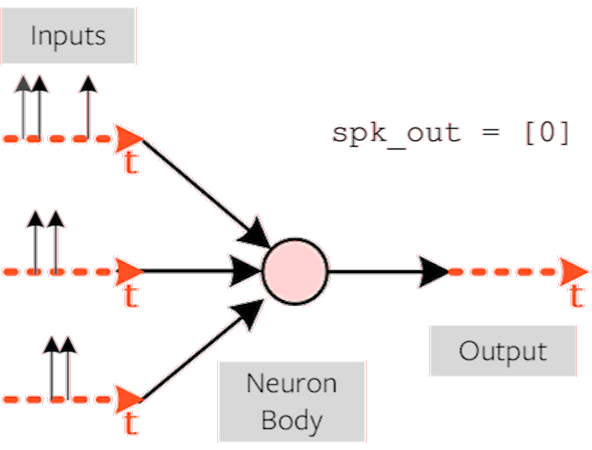
\includegraphics[width=1\textwidth]{image/def1.png}
    \caption{SNN input}
    \label{fig:def1}
  \end{minipage}\hfill
  \begin{minipage}{0.45\textwidth}
    \centering
    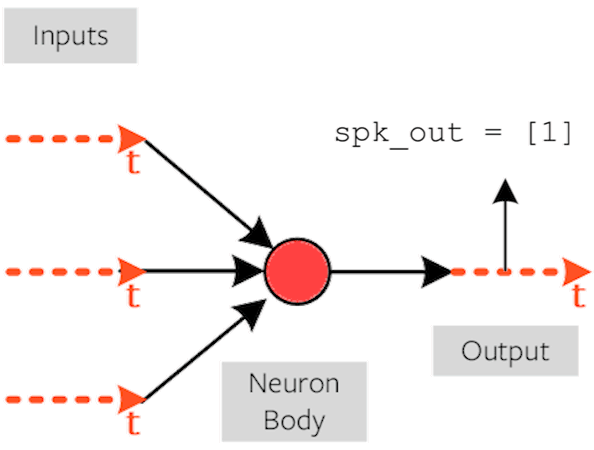
\includegraphics[width=1\textwidth]{image/def2.png}
    \caption{SNN output}
    \label{fig:def2}
  \end{minipage}
\end{figure}

\pagebreak

\subsubsection{Audio classification task}

Audio classification is a fundamental problem in the field of audio processing. It involves assigning a label to an audio clip based on its content. The audio classification task can be further divided into two subtasks: sound event detection (SED) and sound event classification (SEC). SED involves detecting the onset and offset times of sound events in an audio clip, while SEC involves assigning a label to each detected sound event.

In the context of audio classification, training an SNN involves working on image representations of audio data and encoding schemes suitable for SNNs.


\subsubsection{Objectives of the project}

The primary goal of our project is to exploit the temporal processing capabilities of SNNs for audio classification tasks. Specifically, we want to develop models capable of classifying (and possibly detecting) sound events from audio data.

Furthermore, knowing that SNNs consume less power than traditional Artificial Neural Networks (ANNs), but have lower overall accuracy, we want to perform a performance comparison of SNNs with ANNs.

The fullfillment of these objectives would allow us to determine the potential of SNNs for audio classification tasks and to identify the advantages and disadvantages of SNNs compared to other neural networks. Moreover, it is a great way for us to learn more about SNNs and audio classification.

\subsubsection*{aide}
•	Décrire le sujet et résumer votre travail
•	Bien décrire vos contributions et l’intérêt des résultats obtenus


\begin{itemize}
  \item \textbf{Title:} Sound Detection and Classification using Spiking Neural Networks
  \item \textbf{Keywords:} Spiking Neural Networks, Audio Classification, AudioSet, Sound Event Detection, Sound Event Classification
  \item What is a spiking neural network?
  \item How it works ?
  \item Advantages and disadvantages of SNNs compared to other neural networks
  \item What is the goal of the project?
  \item Interrest of the project?
\end{itemize}

\pagebreak

\section{Organizing the project}

\subsection{Main tasks}

During the last full time period, we worked on:

\begin{itemize}
  \item \textbf{A preprocessing pipeline} that allows us to dowload, format and segment the audio part of the Youtube videos composing the Google Audioset audio files into images.
        In order to be efficient, the pipeline needed to be parallelized.
        \subitem After downloading these, it became also necessary to perform some verification on the data, which includes checking the audio file properties (sample rate, number of channels, etc.) and the labels related to the audio files.
  \item \textbf{Finding some correct data augmentation techniques} that can be used to improve the performance of the SNNs.
  \item \textbf{Finding a way to encode the audio data into spikes} that can be used as input for the SNNs.
\end{itemize}

\begin{itemize}
  \item \textbf{Implementing the SNNs} that will be used for the audio classification task.
        \subitem Training the SNNs on the audio data.
  \item \textbf{Implementing the ANNs} that we would compare to the SNNs.
  \item \textbf{Comparing the performance of the SNNs and the ANNs} on the audio classification task.
\end{itemize}


\subsection{Planning and team organization}

\subsubsection{Previous work - full time period}

\begin{figure}[h]
  \centering
  \resizebox{0.85\textwidth}{!}{% Add this line, adjust 0.8 to your preference
  \begin{ganttchart}[
      hgrid,
      vgrid,
      x unit=1.0cm,
      y unit title=0.7cm,
      y unit chart=0.9cm,
      title label font=\footnotesize,
      group label font=\footnotesize,
      milestone label font=\footnotesize,
      bar label font=\footnotesize,
      bar label node/.append style={align=left, text width=3cm}
    ]{1}{12}
  
    \gantttitle{Days}{12} \\
    \gantttitlelist{1,...,12}{1} \\
  
    \ganttgroup{\textbf{Setup and Literature Review}}{1}{1} \\
  
    \ganttgroup{\textbf{Working on the data}}{2}{6} \\
    \ganttbar[bar label node/.append style={align=left},
      bar/.append style={fill=red}]{Download, Format and Segment}{2}{5} \\
    \ganttbar[bar label node/.append style={align=left},
      bar/.append style={fill=blue}]{Data transformation}{2}{6} \\
    \ganttgroup{\textbf{Verification and SnnToch}}{6}{10} \\
    \ganttbar[bar label node/.append style={align=left},
      bar/.append style={fill=red}]{Data Verification and debugging}{6}{9} \\
    \ganttbar[bar label node/.append style={align=left},
      bar/.append style={fill=blue}]{Handling SnnTorch}{7}{10} \\
  
    \ganttgroup{\textbf{First implementations}}{11}{12} \\
    \ganttbar[bar label node/.append style={align=left},
      bar/.append style={fill=red}]{Testing ANNs}{11}{12} \\
    \ganttbar[bar label node/.append style={align=left},
      bar/.append style={fill=blue}]{Develop Spike Encoding}{11}{12} \\
  
  \end{ganttchart}
  }% Add this line
  \caption{Planning of the full time period}
  \label{fig:ftp1}
\end{figure}

\begin{itemize}
  \item Téo : \textcolor{blue}{blue} 
  \item Loaï : \textcolor{red}{red}
\end{itemize}

So far, we have been able to encode and decode the audio data into spikes.

%We were also able to train an ANN on the audio data and test it on the audio classification task. 

Since the first tasks we had to perform would not be connected until they were finished, we decided to work on them in parallel. This allowed us to be more efficient and, most importantly, to save time.

\subsection{Changes in the organization}

In the initial planning, there was no task related to the verification of the data nor to the debugging of part of the code. Each subpart of the preprocessing pipeline part takes a lot of time to be implemented and tested. We had to spend some time debugging the code and verifying the data. 

%Handling the SnnTorch library also took more time than expected.


\subsubsection*{aide}

•	Quelles sont les principales tâches à réaliser ?
•	Décrire brièvement le planning du projet.
•	Décrire comment les membres de l’équipe s’organisent pour faire avancer le PER.
•	Des changements d’organisation ont-ils été nécessaires ?


\begin{itemize}
  \item Tasks
  \item Méthode de travail
  \item Répartition des tâches
  \item Planning
  \item Gestion du projet (au fur et à mesure des difficultés rencontrées)
\end{itemize}

\pagebreak

\section{Technical environment}

\subsection{Computational tools}

We worked on our personal computers and we used the following computational tools: 


\begin{figure}[h]
\begin{center}
  \begin{tabularx}{\textwidth}{|X|X|}
  \hline
  \textbf{Softwares} & \href{https://code.visualstudio.com/}{Visual Studio Code} \\
   & \href{https://jupyter.org/}{Jupyter Notebook} \\
   & \href{https://git-scm.com/}{Git} \\
   & \href{https://github.com/}{Github} \\
   & \href{https://colab.research.google.com/}{Google Colab} \\
    & \href{https://www.anaconda.com/products/individual}{Anaconda} \\
  \hline
  \textbf{Programming languages} 
   & \href{https://www.python.org/}{Python} \\
    & \href{https://www.latex-project.org/}{Latex} \\
  \hline
  \textbf{Libraries} & \href{https://pytorch.org/}{Pytorch} \\
   & \href{https://librosa.org/doc/latest/index.html}{Librosa} \\
   & \href{https://numpy.org/}{Numpy} \\
   & \href{https://pandas.pydata.org/}{Pandas} \\
   & \href{https://matplotlib.org/}{Matplotlib} \\
   & \href{https://pytorch.org/audio/stable/index.html}{sox} \\
   & \href{https://github.com/ytdl-org/youtube-dl}{Youtube-dl} \\
  \hline
  \textbf{Frameworks} & \href{https://github.com/eriksoper/SnnTorch}{SnnTorch} \\
  \hline
  \end{tabularx}
  \end{center}
  \caption{Computational tools}
\end{figure}

\href{https://github.com/LGPolytech/Project_S9}{(Our Github repository)}



\subsection{Documentation}

\subsection{Changing}

\subsubsection*{aide}

•	Environnement informatique, logiciel, notebooks, langage de programmation, etc.
•	Documentation (livres, articles, recherche sur le web, etc.)
•	Des changements dans l’environnement technique ont-ils eu lieu ?

\begin{itemize}
  \item Environnement technique
  \item Logiciels
  \item Langages de programmation
  \item Notebooks
  \item Documentation
  \item Changements dans l'environnement technique
  \item Difficultés rencontrées
  \item Solutions apportées
\end{itemize}

\pagebreak

\section{Description du travail réalisé}

•	Qu’avez-vous produit depuis la fin de la première période à temps plein ?
•	Quels sont vos avancées techniques et/ou théoriques ?
•	Quels sont vos résultats ?


\pagebreak

\section{Difficultés rencontrées}

•	Description des difficultés principales rencontrées durant le projet et des solutions mises en place (si cela était possible).
•	Les commentaires lors de la première soutenance ont-ils été utiles ?

\pagebreak

\section{Conclusion et perspectives}

•	Mettre en valeur votre travail et les domaines où vous avez progressé.
•	Souligner en quoi la formation suivie à Polytech Nice Sophia (ou ailleurs) vous a aidé.
•	Que comptez-vous faire dans les prochaines semaines ?

\pagebreak

\listoffigures

\pagebreak

% Bibliography
\bibliographystyle{siam}
\bibliography{ref}

\end{document}
